%% LaTeX2e class for student theses
%% sections/evaluation.tex
%%
%% Karlsruhe University of Applied Sciences
%% Faculty of  Computer Science and Business Information Systems
%% Distributed Systems (vsys)
%%
%% Prof. Dr. Christian Zirpins
%% christian.zirpins@hs-karlsruhe.de
%%
%%
%% Version 0.2, 2017-11-15
%%
%% --------------------------------------------------------
%% | Derived from sdqthesis by Erik Burger burger@kit.edu |
%% --------------------------------------------------------

\chapter{Evaluation}
\label{ch:Evaluation}
\todo{JMeter Test, welche Endpunkte machen sind getestet zu werden}
Zu Beginn dieses Kapitels werden verschiedenste Anwendungsbeispiele anhand von Diagrammen veranschaulicht und erklärt. Insgesamt werden die folgenden fünf Anwendungsbeispiele beschrieben:
\begin{itemize}
	\item Folgen eines Nutzers aus einem anderen Netzwerk
	\item \glqq Liken\grqq~eines Objekts in einem anderen Netzwerk
	\item Rückgängig machen einer zuvor gesendeten \glqq Follow\grqq~Aktivität
	\item Die Umkehrung eines \glqq Likes\grqq~(Dislike)
	\item Artikel erstellen in einem anderen Netzwerk
\end{itemize}
Des weiteren wird eine Performanz-Messung für die Signatur Erstellung, sowie Verifikation durchgeführt und die Ergebnisse interpretiert. Es wird sich für die Messung der Signatur Erstellung sowie Verifikation entschieden, da diese beiden Schritte eine nicht geringe Zeit der gesamten Anfrage in Anspruch nehmen. Damit wird versucht eine Hilfestellung für verschiedene Situationen zu bieten. Wird z. B. auf die Performanz großen Wert gelegt, kann anhand der Ergebnisse die Entscheidung für eine Hashfunktion gefällt werden.\\

Bei der Messung werden 4 verschiedene Ergebnistabellen erstellt; Jeweils zwei für eine Hardwarevariation. Zum Einen wird ein älteres Notebook Modell zum testen verwenden, zum Anderen ein Spiele-Computer. Außerdem wird aufgrund der interpretierten Ergebnisse und anderen Aspekten Empfehlungen gegeben, welche Hashfunktion für welchen Zweck am Besten passt.
\section{Anwendungsbeispiel}
Bei jedem der folgenden Anwendungsbeispiele muss sich der Server mit einer HTTP Signatur authentisieren. Die Signaturen werden beim ActivityPub Protokoll mit dem privaten Schlüssel des interagierenden Nutzers erstellt und mit dem öffentlichen verifiziert. Im folgenden Diagramm wird das ersichtlich durch den Anwendungsfall \glqq HTTP Signatur verifizieren\grqq, welcher im Empfangen von Aktivitäten beinhaltet ist:\\
\begin{figure}[h]
	\begin{minipage}{\textwidth}
		\centering
		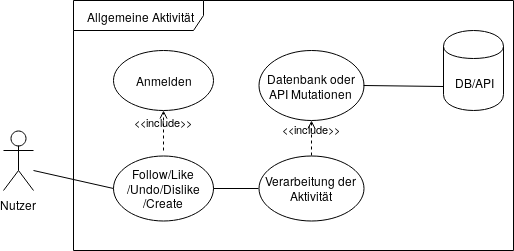
\includegraphics[scale=0.75]{figures/generel-activity-usecase.png}
		\label{fig:generel-activity-usecase}
		\caption{Generelles Anwendungsfalldiagramm für das Empfangen von Aktivitäten}
	\end{minipage}
\end{figure}

\textbf{Beispiel 1} (Nutzer wird gefolgt):\\
Eine Nutzerin Alice aus einem anderen Netzwerk oder von einer anderen Instanz des selben Netzwerks, genannt Instanz A, möchte einem Nutzer auf Instanz B folgen. Dafür muss Alice dem zu folgenden Nutzer Bob über die Suchfunktion auf Instanz A finden und anschließend auf den \glqq folgen\grqq~Knopf drücken. Dadurch wird auf der Instanz A eine Anfrage erstellt, welche mit dem privaten Schlüssel von Alice signiert wird. Trifft die signierte Anfrage bei Instanz B ein wird zuerst die Signatur mit dem öffentlichen Schlüssel von Alice geprüft. Bei einer erfolgreichen Verifikation wird die Anfrage weiter verarbeitet und vom Server entsprechend eine \glqq Accept\grqq~oder \glqq Reject\grqq~Aktivität gesendet. Schlägt die Signatur-Prüfung fehl wird ein \glqq Forbidden\grqq~Statuscode zurückgegeben.\\

Auch in den folgenden Beispielen werden die Benutzer Alice und Bob als Beispielnutzer genannt welche entsprechend auf Instanz A (Alice) und Instanz B (Bob) residieren.\\

\textbf{Beispiel 2} (Rückgängig machen eines vorherigen folgens):\\
Da sich Alice und Bob gestritten haben möchte Alice keine weiteren Benachrichtigungen von Bob erhalten, deshalb folgt Sie Bob nun nicht mehr. Instanz A erstellt, signiert und sendet somit eine Anfrage mit einer \glqq Undo\grqq~Aktivität an Instanz B.\\

\textbf{Beispiel 3} (Objekt eines Nutzers \glqq liken\grqq):\\
Alice durchsucht ihre Zeitleiste nach neuen Inhalten. Sie stößt auf einen Inhalt von Bob, den Sie sehr mag. Daraufhin \glqq liked\grqq~Sie den Inhalt. Instanz A erstellt eine \glqq Like\grqq~Aktivität und signiert diese mit Alice ihrem privaten Schlüssel. Die Anfrage wird nun auf Empfängerinstanz B verifiziert und, bei Erfolg, verarbeitet.\\

\textbf{Beispiel 4} (Rückgängig machen eines vorherigen \glqq likes\grqq):\\
Der zuvor von Alice gemochte Inhalt wurde in der Zwischenzeit von Bob verändert. Alice sieht dies, liest den Inhalt erneut und wundert sich warum Bob den Inhalt verändert hat. Ihrer Ansicht nach war er vorher viel Aussagekräftiger, daher \glqq Disliked\grqq~Sie den Inhalt.\\

\textbf{Beispiel 5} (Erstellen eines Inhalts):\\
Nach einem schönen Wochenende möchte Alice ihre neuen Erfahrungen in einem Inhalt zusammenfassen und an ihre Freunde senden. Sie meldet sich bei Instanz A an und verfasst ihre Erfahrungen. Nach dem absenden erstellt Instanz A eine \glqq Create\grqq~Aktivität mit einem Artikel als Objekt und sendet signierte Anfragen an jeden ihrer Freunde.
\todo{Einzelne Testfälle vorstellen und aufzeigen das sie funktionieren}
\todo{HTTP Anfragen anzeigen}
\todo{Anwendungsbeispiele Applikation selbst}
\section{Performanz-Messungen}
\todo{Performanz Messung mit JMeter}
Es wurde die Performanz der Erstellung von Signaturen, sowie der Verifikation solcher gemessen.

Insgesamt wurden 2 Messungen mit je 10 Testdurchläufen pro Hashfunktion durchgeführt. Die erste Messung wurde auf einem Notebook mit eingebauter Intel 2-Kern \gls{cpu} der Serie Core i5 und einer Taktfrequenz von 2,4 GH durchgeführt\footnote{\url{https://ark.intel.com/content/www/de/de/ark/products/47341/intel-core-i5-520m-processor-3m-cache-2-40-ghz.html}}. Bei der zweiten Messung kam eine 16-Kern AMD \gls{cpu} aus der \glqq Ryzen\grqq~Serie mit der Bezeichnung \glqq Threadripper 2950X\grqq~und einer Taktfrequenz von 3,5 GH zum Einsatz\footnote{\url{https://www.amd.com/de/products/cpu/amd-ryzen-threadripper-2950x}}.\\
\todo{Performanz-Messung in die Implementierung verschieben}
Die Performanzmessungen wurden in der Node.js Laufzeitumgebung mit der Version 10.15.3 durchgeführt unter Zuhilfenahme der internen process.hrtime() Funktion. Diese wird vor und nach dem Erstellen sowie Verifizieren aufgerufen. Die Rückgabe des zweiten Aufrufs nach der jeweiligen Funktion enthält die Differenz zum ersten Aufruf in Nanosekunden.
\begin{table}[h]
	\begin{tabularx}{\textwidth}{p{0.15\textwidth}|X|X|X|r}
		& RSA-MD4 & RSA-MD5 & RSA-SHA256 & RSA-SHA512\\
		\hline
		Testlauf 1& 24.254 ms& 24.123 ms& 24.171 ms& 24.173 ms\\
		Testlauf 2& 22.833 ms& 23.006 ms& 23.626 ms& 22.948 ms\\
		Testlauf 3& 27.186 ms& 23.113 ms& 22.873 ms& 22.781 ms\\
		Testlauf 4& 23.630 ms& 24.256 ms& 22.597 ms& 22.667 ms\\
		Testlauf 5& 25.012 ms& 24.027 ms& 24.343 ms& 30.278 ms\\
		Testlauf 6& 30.221 ms& 23.032 ms& 22.827 ms& 22.768 ms\\
		Testlauf 7& 27.050 ms& 29.950 ms& 22.629 ms& 22.774 ms\\
		Testlauf 8& 23.630 ms& 24.282 ms& 24.625 ms& 25.495 ms\\
		Testlauf 9& 23.151 ms& 22.958 ms& 22.854 ms& 26.816 ms\\
		Testlauf 10& 22.654 ms& 24.067 ms& 23.637 ms& 23.579 ms\\
		\hline
		Arithmetisches Mittel& 25,122 ms& 24,281 ms& 23,418 ms& 24,427 ms\\
	\end{tabularx}
	\caption{Testergebnisse der ersten Messung (Signatur Erstellung)}
\end{table}
Beim betrachten der arithmetischen Mittel fällt auf, dass die Messwerte sehr nahe beieinander liegen. Die SHA256 Hashfunktion schneidet dabei mit einer Funktionslaufzeit von 23,418 ms am Besten ab. Auf Platz zwei liegt die MD5 Funktion mit 24,281 ms gefolgt von SHA512 mit 24,427 ms. Das Schlusslicht bildet MD4 mit einer Laufzeit von 25,122 ms.\\
Aus Sicht der Performanz wird bei der ersten Messung somit die SHA256 Hashfunktion zur Signierung empfohlen.
\begin{table}[h]
	\begin{tabularx}{\textwidth}{p{0.15\textwidth}|X|X|X|r}
		& RSA-MD4 & RSA-MD5 & RSA-SHA256 & RSA-SHA512\\
		\hline
		Testlauf 1& 107,177 ms& 128.993 ms& 121.406 ms& 114.669 ms\\
		Testlauf 2& 43,660 ms& 51.178 ms& 35.524 ms& 39.633 ms\\
		Testlauf 3& 32.101 ms& 32.691 ms& 30.461 ms& 32.293 ms\\
		Testlauf 4& 36.096 ms& 30.279 ms& 32.018 ms& 43.842 ms\\
		Testlauf 5& 31.869 ms& 34.882 ms& 30.877 ms& 26.555 ms\\
		Testlauf 6& 39.218 ms& 67.507 ms& 38.734 ms& 31.330 ms\\
		Testlauf 7& 40.996 ms& 39.646 ms& 45.433 ms& 27.290 ms\\
		Testlauf 8& 25.977 ms& 39.302 ms& 26.778 ms& 53.478 ms\\
		Testlauf 9& 23.641 ms& 37.833 ms& 30.485 ms& 36.284 ms\\
		Testlauf 10& 31.097 ms& 52.725 ms& 28.943 ms& 28.634 ms\\
		\hline
		Arithmetisches Mittel& 41,183 ms& 51,503 ms& 42,065 ms& 43,400 ms
	\end{tabularx}
	\caption{Testergebnisse der ersten Messung (Signatur Verifikation)}
\end{table}
Werden die Arithmetischen Mittel der Verifikation betrachtet ist eine Zeitspanne von 10 ms Sekunden zu Beobachten in welcher sich alle Messwerte befinden. Dabei ist der MD4 Algorithmus mit 41,183 ms auf Position eins, während sich MD5 mit 51,503 ms auf der letzten Position befindet. Die beiden Funktionen SHA256 und SHA512 liegen mit Laufzeiten von 42,065 und 43,400 ms näher an der MD4 Funktion. Zudem fällt auf, dass bei der Verifikation die ersten Messwerte stark abweichen von allen weiteren. Das ist dadurch zu erklären, dass zuerst eine HTTP Anfrage gesendet werden muss um den benötigten öffentlichen Schlüssel zu erhalten. Jegliche weitere Anfragen werden aus dem Cache bedient und sind somit um einen groben Faktor von 2 schneller als die erste Anfrage.\\
\begin{table}[h]
	\begin{tabularx}{\textwidth}{p{0.15\textwidth}|X|X|X|r}
		& RSA-MD4 & RSA-MD5 & RSA-SHA256 & RSA-SHA512\\
		\hline
		Testlauf 1& 7.152 ms& 7.137 ms& 8.178 ms& 7.002 ms\\
		Testlauf 2& 6.955 ms& 7.134 ms& 6.714 ms& 7.048 ms\\
		Testlauf 3& 6.910 ms& 6.762 ms& 6.703 ms& 6.860 ms\\
		Testlauf 4& 7.044 ms& 6.800 ms& 6.827 ms& 6.982 ms\\
		Testlauf 5& 6.935 ms& 7.831 ms& 6.854 ms& 6.958 ms\\
		Testlauf 6& 7.191 ms& 7.697 ms& 6.873 ms& 7.050 ms\\
		Testlauf 7& 7.195 ms& 7.108 ms& 6.728 ms& 6.840 ms\\
		Testlauf 8& 7.237 ms& 6.864 ms& 6.743 ms& 6.722 ms\\
		Testlauf 9& 7.136 ms& 7.016 ms& 6.740 ms& 6.834 ms\\
		Testlauf 10& 7.128 ms& 6.939 ms& 6.811 ms& 6.819 ms\\
		\hline
		Arithmetisches Mittel& 7,088 ms& 7,128 ms& 6,917 ms& 6,911 ms
	\end{tabularx}
	\caption{Testergebnisse der zweiten Messung (Signatur Erstellung)}
\end{table}
Anders als bei der ersten Messung liegt bei Betrachtung der arithmetischen Mittel keine Zeitspanne vor, sondern die Messwerte liegen sehr nahe beieinander. Dabei ist die SHA512 Hashfunktion am schnellsten mit 6,911 ms, dicht gefolgt von der SHA256 Funktion mit einer Laufzeit von 6,917 ms. Auf Platz drei ist die MD4 Funktion mit 7,088 ms und auf Platz vier MD5 mit 7,128 ms.\\
\begin{table}[h]
	\begin{tabularx}{\textwidth}{p{0.15\textwidth}|X|X|X|r}
		& RSA-MD4 & RSA-MD5 & RSA-SHA256 & RSA-SHA512\\
		\hline
		Testlauf 1& 45.639 ms& 50.422 ms& 53.230 ms& 50.732 ms\\
		Testlauf 2& 16.919 ms& 18.139 ms& 15.841 ms& 16.793 ms\\
		Testlauf 3& 19.744 ms& 12.443 ms& 15.318 ms& 16.947 ms\\
		Testlauf 4& 18.103 ms& 14.628 ms& 15.803 ms& 13.946 ms\\
		Testlauf 5& 16.982 ms& 13.784 ms& 13.126 ms& 12.239 ms\\
		Testlauf 6& 18.338 ms& 14.137 ms& 24.549 ms& 19.943 ms\\
		Testlauf 7& 14.566 ms& 11.247 ms& 11.772 ms& 12.191 ms\\
		Testlauf 8& 17.689 ms& 13.369 ms& 12.277 ms& 16.769 ms\\
		Testlauf 9& 13.462 ms& 14.808 ms& 11.173 ms& 14.314 ms\\
		Testlauf 10& 15.422 ms& 16.029 ms& 12.069 ms& 12.693 ms\\
		\hline
		Arithmetisches Mittel& 18,144 ms& 17,900 ms& 18,515 ms& 18,656 ms
	\end{tabularx}
	\caption{Testergebnisse der zweiten Messung (Signatur Verifikation)}
\end{table}
Wie auch in der ersten Messung sehen wir bei der Verifikation, dass die beginnenden Messwerte einen deutlichen Unterschied zu weiteren aufweisen. Der Grund ist derselbe wie bei der ersten Messung. Betrachten wir die arithmetischen Mittel, sehen wir Messwerte innerhalb einer Zeitspanne von ungefähr 3 ms in der sich die Messwerte bewegen. Die MD5 Hashfunktion schneidet hierbei am Besten ab mit einer Zeit von 17,900 ms, gefolgt von der MD4 Funktion mit 18,144 ms. Die Schlusslichter bilden hier SHA256 mit 18,515 ms und SHA512 mit 18,656 ms.\\

Wird bei der Erstellung und Verifikation auf die Laufzeit Wert gelegt, gelten folgende Empfehlungen:
\begin{itemize}
	\item Bei der Betrachtung von Messung eins der Signatur Erstellung kann die SHA256 Funktion und von Messung zwei SHA512 empfohlen werden.
	\item Wird die Signatur Verifikation betrachtet, kann die MD4 Funktion bei der ersten Messung und MD5 bei der zweiten empfohlen werden.
\end{itemize}
Aus Sicht der Sicherheit sei allerdings gesagt, dass die Funktionen MD4 und MD5 als unsicher gelten. Da SHA-1 auch die MD4 Funktion verwendet und diese bereits als unsicher gilt, ist somit auch SHA-1 nicht sicher (Vgl. \cite[S. 103]{kryptographie}). Wird also Wert auf kollisionsfrei erzeugte Hashes gelegt, sollte zulasten der Laufzeit vorzugsweise die SHA256 oder SHA512 Funktion Verwendung finden (Vgl. \cite[S. 40, Tabelle 4.1]{bsi-empfehlungen}).
\section{Diskussion von Vor- und Nachteilen der Lösung}
